\lhead{\emph{State of the Art}}

% ***************************************************************************
\chapter{State of the Art}
% ***************************************************************************


% ***************************************************************************
\section{Marker detection}
% ***************************************************************************

The registration technique currently used in this project is the detection of \acrshort{ar} marker in the color image. AR markers are black and white, grid-like patterns developped for augmented reality usage to detect easily a position in space from an RGB camera. \\
This detection is not very accurate but by repeating the process hundreds of time and averaging we can get a good estimation of the position of the cameras. An obvious drawback regarding our needs for this project is the involvement of the user and the equipment requirement. The user need to place a printed pattern into the overlapping region and no other work can be done while performing the registration. \\
To perform this registration we place the marker in the overlapping region so that both camera can be calibrated from this marker (fig. \ref{fig:ar_marker}). As we have already discussed, the overlapping region cannot be trusted due to its poor quality and small size. This can be solved by calibrating both cameras with a different marker position (in the middle of the camera view), these positions have now to be know if we want to match point clouds together. This is a high constraint both for the user to perform the calibration twice and the workspace to be designed such that we can easily move the marker in it while still knowing exactly the position of the marker. This is the reason we are searching for a more automatic registration process for this project. \\

\begin{figure}[h!]
    \centering
    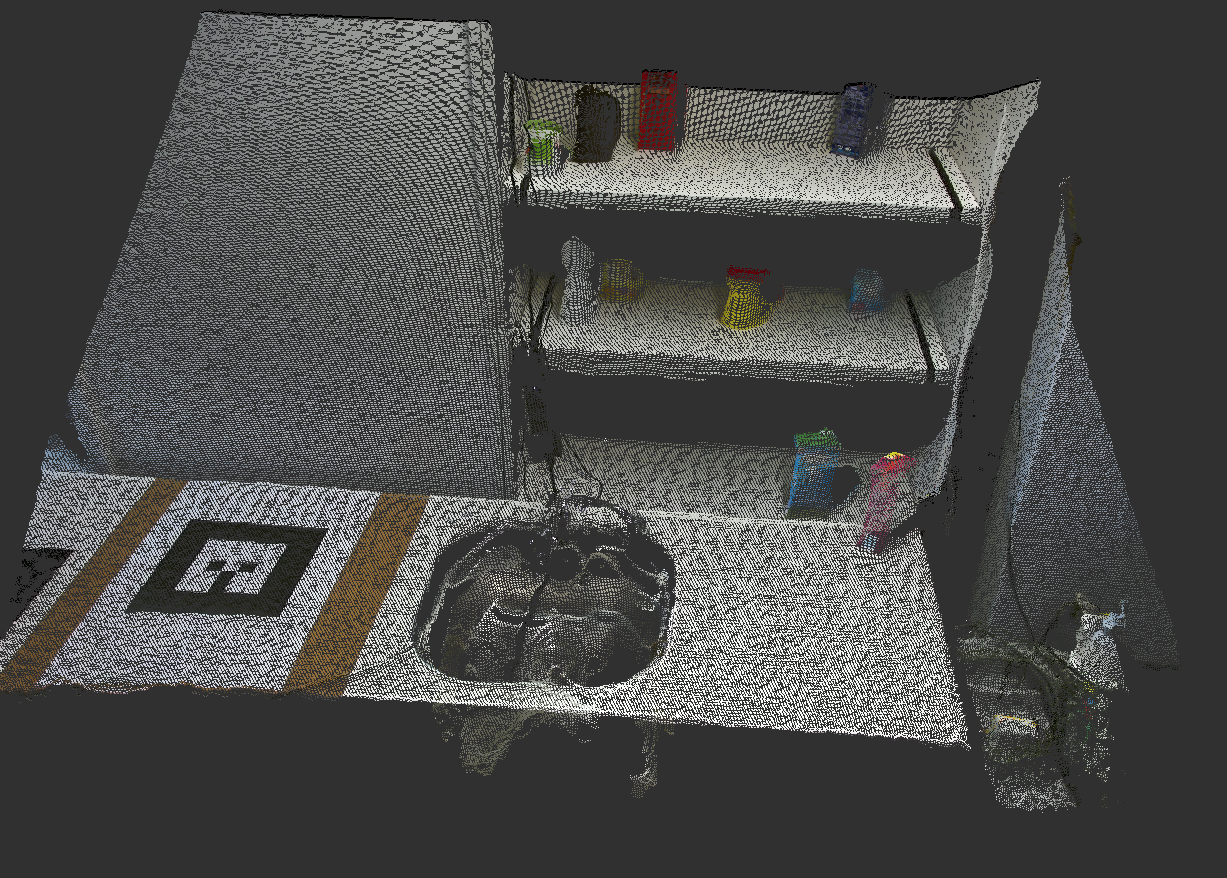
\includegraphics[width=\textwidth]{images/marker_detection.png}
    \caption{AR Marker detection.}
    \label{fig:ar_marker}
\end{figure}

For the implementation, we are using an existing ROS package based on alvar, which tracks AR printed patterns in a color image to estimate its position with respect to this camera. By filming a marker which position in the scene is known with a fix camera, we can average the pose estimation on hundreds of frames to get a good estimation of the actual position of the camera. \\
The main drawback of this technique are the need of printed pattern, human action, time of computation and knowledge of the scene. This is still a good technique to establish our ground truth and to build the entire scene point cloud we could need for other methods as ICP.


% ***************************************************************************
\section{\acrlong{icp}}
% ***************************************************************************

The \acrlong{icp} algorithm is a well known registration algorithm that aims to register 2 point clouds that represent the same objects using an iterative process. These iterations rely on identifying closest points from both point clouds at each step in order to estimate a transformation that will improve the clouds matching without taking account of distant points (considered as outliers).\\

The first step of this algorithm is to find matches between points from the source point cloud $\mathcal{P_S}$ to points in the target cloud $\mathcal{P_T}$. As we have no knowledge of which point within the target cloud should match with source points the key idea is to match source points with their closest neighbors in the target cloud (fig. \ref{fig:closest_point}). After filtering duplicate matches we have pairs of matching points with indices $m_S$ and $m_T$. At this step we define the objective function $f$ which is the \acrshort{mse} of these matches according to the current guess for the rigid transform $\mathcal{T}_{i}$. \\
\[
    f(\mathcal{T}_i) = MSE(\mathcal{P}_T^{m_T} - \mathcal{T}_i\: \mathcal{P}_S^{m_S})
\]
Where the initial guess $\mathcal{T}_0$ should be provided to the program, the quality of this guess will affect the final result. \\
After that we can compute the transform that minimize $f$ for this set of matches. Having a new estimation of the rigid transform, we can repeat the process until convergence. 

\begin{figure}[h!]
    \centering
    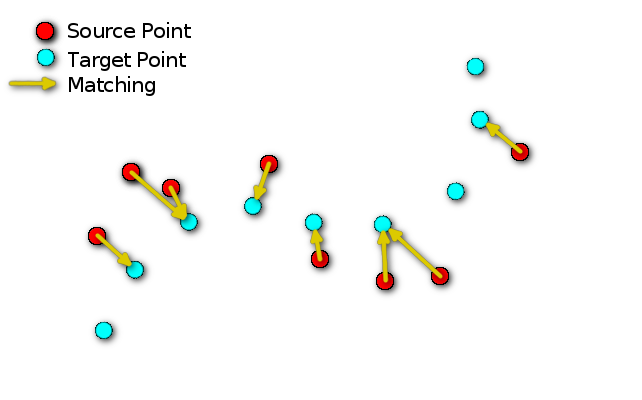
\includegraphics[width=\textwidth]{images/closest_point.png}
    \caption{ICP closest point matching.}
    \label{fig:closest_point}
\end{figure}

The main drawback of this technique come from the need of an initial guess, the \acrshort{icp} algorithm is used for refinement once we have a rough idea of the desired result. This is a problem in our case because we have no previous knowledge over the camera positions and orientation. It could be fixed by using accelerometers for example but the translation part would need a large overlapping region to be solved. This algorithm is indeed highly sensitive to the ratio of overlapping between point clouds. In our case, the low overlapping makes this techniques unusable, even if the registration converge to a coherent result (small translation error), the lack of overlapping, the noise and deformation would not allow to have an accurate estimation of the rotation between clouds which have dramatic effect on low-overlapping point clouds (2 sets of points with a similar centroids would be much less affected by rotation errors). \\
This algorithm also requires a huge amount of computation power if running directly on kinect point clouds which contains more than 16 million points. To run this algorithm faster we have, apart from decreasing the number of iteration and the convergence threshold, to downsample point clouds before running the algorithm. It may decrease the precision of the transform estimation but has no incidence on the final point cloud density since I can simply use the downsampled cloud to estimate the transform and then apply it to the full point cloud.\\
\newline
To perform registration using the ICP method, I am using the PCL implementation of this algorithm. As expected, applying this algorithm with our 2 low overlapping point clouds ends up to really bad results (fig. \ref{fig:icp_cams}), however this technique is more effective when registering a partial view of the scene with a complete model of it (fig. \ref{fig:icp_cams}). I was then able to apply ICP to both point clouds to register them to a more complete 3D model of the scene. This works both when applied to registration with a CAD model of the kitchen and to a complete point cloud generated by merging both kinect views but even with this model we don't have enough information to fix accurately the Y translation (green axis in fig. \ref{fig:ar_marker}). \\

\begin{figure}[h!]
    \centering
    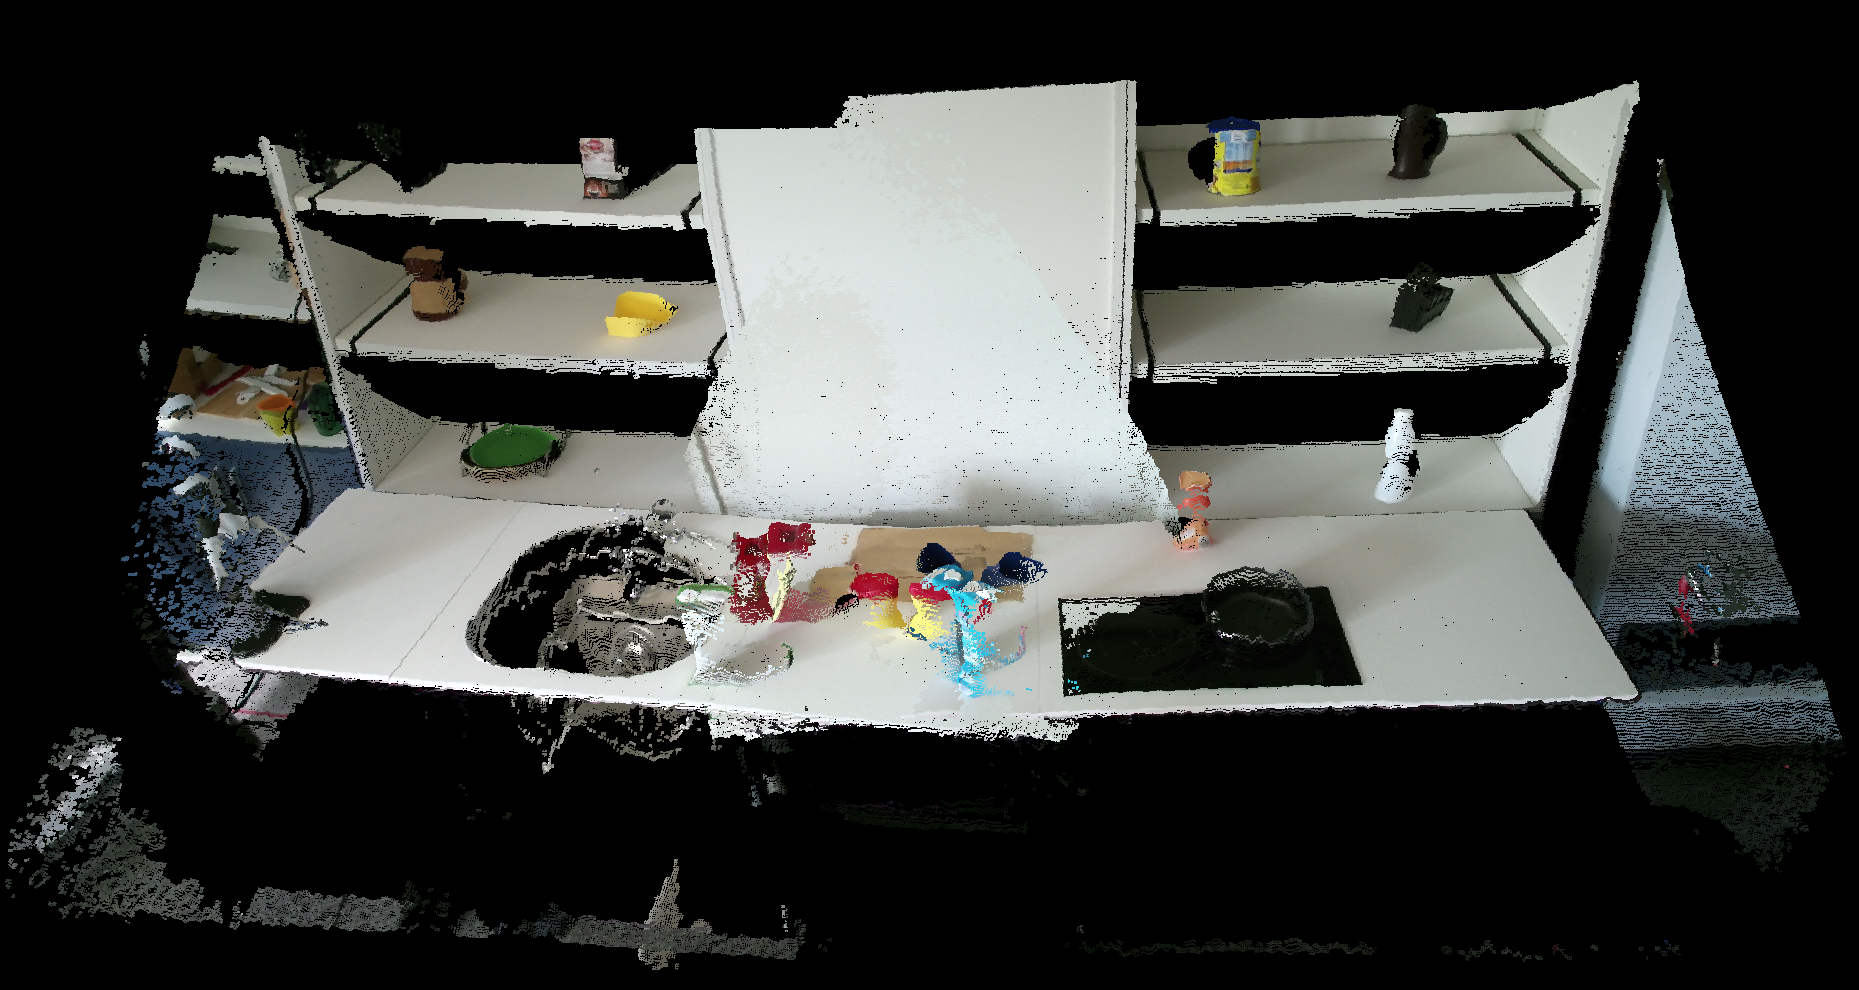
\includegraphics[width=\textwidth]{images/icp_one_one_registration.png}
    \caption{ICP applied to both cameras.}
    \label{fig:icp_cams}
\end{figure}

\begin{figure}[h!]
    \centering
    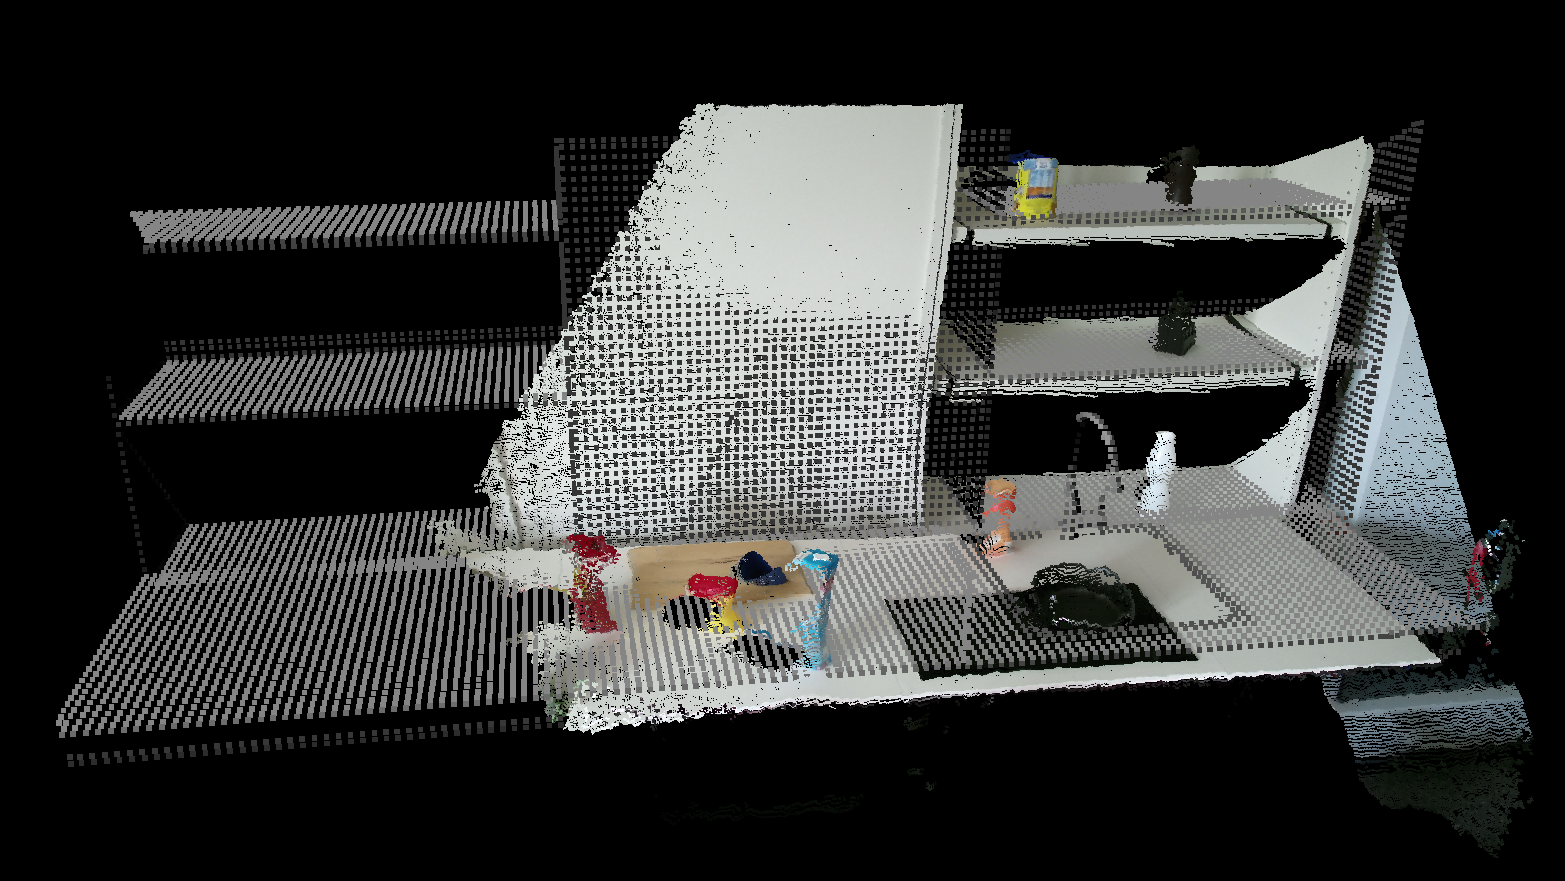
\includegraphics[width=\textwidth]{images/icp_model.png}
    \caption{ICP applied to one camera and a 3D model of the kitchen.}
    \label{fig:icp_model}
\end{figure}

This algorithm is then useful when point clouds have a large overlapping or if we have previously built a model of the scene. As we are not assuming any knowledge on the environment (else than being indoor) and due to the low overlapping of our point clouds, this technique will not be used for the first registration of kinects. This can still remains a good registration method as soon as we have created a complete and reliable model of the scene.

% ***************************************************************************
\section{3D Keypoints}
% ***************************************************************************

An other commonly used registration technique consists in 3D keypoints detection and matching. 
There are a lot of different ways to perform registration using 3D points matching, but the process pipeline is usually similar as the following:

\subsection{Keypoints extraction}

    Input point clouds contains way too much points to run the entire process on all of them. It is thus required to select only a subset of them, we call these selected points, keypoints. As explained in \cite{pcl_feat}, we can use several different keypoints extraction techniques such as \acrshort{iss}, \acrshort{narf} or uniform sampling. \\

\subsection{Features extraction}

    There are a lot of different features we can extract from keypoints but it basically consists in stacking 3D shape and/or color histograms into a vector descriptor, if this descriptor is local, it can then be used to match the most similar keypoints to identify similar points (ie. that represent the same real point in space) from both clouds. This matching process means that this method is also relying only on overlapping regions to perform registration. \\
    For each keypoint, we want to be able to find the most similar keypoint in the second cloud, so it is needed to describe the point surrounding in a way that is invariant to rotation (its equivalent point in the other cloud is probably oriented differently unless both clouds are yet aligned) and translation (scale invariant is not a property we are interested here since we assume cameras are calibrated). This description is usually based on geometric features (relative position or density of its neighbors) and/or color features (color distribution around the point).
    
\subsection{Matching}

    These descriptors can now be metched by finding a coherent measure of distance within the chosen descriptor space so that a small distance between descriptors means that the corresponding points are similar.
    
\subsection{Outliers Rejection} 

    It is then often required to refine the previous matching by eliminating undesired matches such as if several points are matching with the same target point (we'll then keep only the best match, ie. with the smallest descriptor distance), called duplicates, points that are too far (in space) according to the initial guess or points with descriptor distance over a given threshold.
    
\subsection{Transform Estimation} 
    
    The last step is then to estimate the transform that brings source matched points to their corresponding target points.


To apply this pipeline, I used the PCL implementation of these algorithms. I am using SHOT features which contains information on both geometry of the surrounding of the keypoint and color distribution. 
... \\
The resulting quality of this technique depends on matches accuracy (and successful matching ratio) but also on their spreading since the same error will produce a lower registration angle error if the keypoints matched are more distant. This, this algorithm will only be useful when a large part of the clouds is overlapping, in our case this method can't be applied.

% ***************************************************************************
\section{Plane detection}
% ***************************************************************************

An other interesting method that can be found in some papers is based on plane detection and matching. This method can solve the issue caused by low overlapping. Indeed, planes can be used to estimate how to merge the point clouds so that the overlapping region is continuous, but the interesting property is that the plane equation can be computed with every point that lies into the plane model whether it is in the overlapping region or not. Thus, if the cloud contains large plains that can be identified with a large number of points spread in a large part of the point cloud, the confidence on this plane's equation will be far better than if we try to identify features in the overlapping region. \\
However, to determine the whole 6 degrees of freedom of the transformation between camera positions, we would need 3 non-degenerate planes (ie. which normals describe a basis, the more orthogonal the better) to match in both point clouds. This condition is often too constraining to be satisfied, or is satisfied only if considering small and/or almost degenerate sets of planes. In this case, the accuracy gain provided by the plane identification is lost and one degree of freedom is left with a lot of uncertainty. Nevertheless, in most cases we can at least fix quite accurately the rotation between clouds (2 planes needed). \\
To apply this technique, I have used PCL's RANSAC implementation in order to achieve plane detection. Similarly to the previous registration method, the next step consists in matching extracted planes. \\
My first try was to match using feature matching in the same way as I did with keypoints descriptors but using global descriptors (descriptors that contains information on the entire plane). However, due to the similarity of planes in this particular scene (here, every planes is detected as an almost entirely white rectangle which fails the matching algorithm most of the time). Another technique could be to simply use brute force, since we are usually not trying to detect a lot of planes (we need 3 of them), by trying every possible matching we could make sure to keep the one that ends with the best registration result. Nevertheless this technique should better be applied to improve the matching after the whole registration process is implemented and optimized to reduce the computation speed, otherwise, repeating the process for every 6 matching possibilities may be too demanding. \\
For this reason I preferred to match planes by normal similarity, this technique doesn't rely on the later use of plane matches and is simple to implement. The only requirement is not to have a huge orientation difference between cameras. We may want to eliminate this assumption later but, for testing and comparison purpose, this method should be sufficient because it is highly reliable under this assumption and requires few computations. \\
The last step is to estimate the rigid transform that minimize plane-to-plane matching error as suggested in \cite{khoshelham2016}. 
\newline
If we define a plane as the vector $\pi=(n^T, -\rho)$ (normal vector and distance to origin) that satisfy for every point $p$ of this plane the equation:
\[\pi p=0\]
And let $H$ be the transform between point clouds A and B such that:
\[p^B = Hp^A\]
We can define $H'$ the transform that brings any plane equation in A $\pi^A$ to its corresponding plane in point cloud B $\pi^{B}$. We can demonstrate that: \[H'=H^-T\]
Finding $H$ is then the same as finding $H'$ that minimize plane distances: \[\pi^B_i=H'\pi^A_i\]
If we write:
\[H'=\begin{bmatrix}
R & t\\ 
0 & 1
\end{bmatrix}\]
We then have for each matching planes:
\[\left\{\begin{matrix}
{n_i^B}^TR={n_i^A}^T\\ 
{n_i^B}^Tt=\rho_i^B-\rho_i^A
\end{matrix}\right.\]
By stacking all $n$ vectors into a matrix $N$ and all $\rho_i^B-\rho_i^A$ into a vector $d$, the problem became:
\[\left\{\begin{matrix}
N^BR=N^A\\ 
N^Bt=d
\end{matrix}\right.\]
We can then simply compute the least square solutions for any n-dimensional distance metric where n is the number of matches. Especially, a useful metric could be for any n-d weight matrix $W$:
\[\mathcal{D}(x,y)=a^TWb\]
This metric will allow to weight some planes differently according to the confidence we give to the precision of their plane detection, otherwise $W=I_n$ will be used.
The final solution is:
\[\left\{\begin{matrix}
\tilde{t}=({N^B}^TWN^B)^{-1}{N^B}^TWd\\ 
\tilde{R}=({N^B}^TWN^B)^{-1}{N^B}^TWN^A
\end{matrix}\right.\]

At the end we can then ensure the orthogonality of $R$ using SVD decomposition. \\

The main limitation of this technique is that the scene needs to have large planes in it, but it is really common in indoor environments. However, having 3 large matching planes is lot more difficult, this is again an indirect consequence of the lack of overlapping. To identify 3 planes means that the sensor is seeing a corner but it is not probable being able to see this corner in both views if the overlapping is small, moreover even if we do, the corner will be in the border of both view, meaning at least one plane will be small. To summarize, we can't expect to detect required planes by luck. We may be able to use this algorithm in some specific cases but it is not possible to plan to use it if we don't have knowledge of the scene.